\documentclass[12pt,a4paper]{ufpr}

% \usepackage[portuges,brazil]{babel}
% \usepackage[portuguese,brazil]{babel}

%\usepackage[brazil]{babel}
\usepackage[utf8x]{inputenc}
\usepackage[T1]{fontenc}
\usepackage{amssymb,amsmath}
\usepackage{epsfig}
\usepackage{multirow}
\usepackage{algorithm}
\usepackage{algorithmic}


\usepackage{eqparbox}
\renewcommand{\algorithmiccomment}[1]{\hfill\eqparbox{COMMENT}{\# #1}}


\usepackage{amssymb}
\usepackage{subfigure}
\usepackage{graphicx}
\usepackage{caption2}
\usepackage{setspace}
\usepackage{ps-macros}
% \usepackage{psfig}

\setcounter{secnumdepth}{3}    % n - numero de niveis de subsubsection numeradas
\setcounter{tocdepth}{3}       % coloca ate o nivel n no sumario

%%% add agora

\graphicspath{{./images/}}




%% fim

\title{Improved resource consolidation for database workloads in a cloud}
\author{Antonio Carlos Salzvedel Furtado Junior}
\advisortitle{Orientator} % ou Orientador
\advisorname{Prof. Dr. Eduardo Almeida}
\advisorplace{Department of Informatics, UFPR}  % departamento, instituicao
\city{Curitiba}
\year{2011}

%\banca        % nao insira o nome do orientador, ja eh feito automaticamente
%{Prof. Dr. Educardo Almeida}{Departamento de Inform?tica, UFPR} % se nao houver deixe em branco {}{}
%{}{}    % se houver um quarto membro na banca, inserir nome e instituicao

\defesa{} % dia em que foi realizada a defesa da dissertacao


\begin{document}

%\makecapaproposta             % cria capa para proposta%
\makecapadissertacao           % cria capa para dissertacao de mestrado %
\makerosto                     % cria folha de rosto para versao final da UFPR %
%\maketermo                     % cria folha com o termo de aprovacao da dissertacao%

%\singlespacing           % espacamento 1 - capa UFPR%
%\onehalfspacing          % espacamento 1/2 %
\doublespacing            % espacamento 2 - UFPR %

\pagestyle{headings}
\pagenumbering{roman}

%\chapter*{Agradecimentos}
%\input{agradecimentos.tex}          % possiu somente o texto

\tableofcontents

%\listoffigures         % se houver mais do que 3 figuras
%\addcontentsline{toc}{chapter}{\MakeUppercase{Lista de Figuras}}
%\newpage

%\listoftables        % se houver mais do que 3 tabelas
%\addcontentsline{toc}{chapter}{\MakeUppercase{Lista de Tabelas}}
%\newpage


\chapter*{Abstract}
\addcontentsline{toc}{chapter}{\MakeUppercase{Abstract}}
Cloud computing has attracted a lot of attention, both in researches and as a business model. It promises a lot of benefits, which include the possibility of cutting costs, better manageability of applications, better utilisation of computational resources, among others. In order to achieve its goals, the cloud is highly dependable on the virtualization of resources to provide its elasticity. At the same time, the demand for running database systems in virtualized environments grows. Database systems running in the cloud has already been debated by some recent papers.

Database systems have particularities involving their workloads, when compared to regular applications. This raises some questions about how to optimize the resource allocation among database workloads in a elastic cloud environment. In this paper, we propose an implementation of a \textit{virtual design advisor} in the cloud. Its goal is to improve the resource allocation among database management systems running inside virtual machines, by recommending configuration parameters for them. It bases its recommendations on database cost models.        % somente o texto
\newpage


\pagenumbering{arabic}

\chapter{\textbf{Introduction}}

\label{Introduction}

Cloud computing has attracted a lot of attention lately. It was popularized as a business model by Amazon's Elastic Compute Cloud (EC2), which started selling virtual machines (VMs) in 2006. Over time, more cloud providers have appeared in the market, offering their computational resources (CPU, memory, and I/O bandwidth). This definition of cloud, in which the IT infrastructure is deployed through virtual machines, is referred as Infrastructure-as-a-service (IaaS). One of the most appealing benefits of this paradigm, when associated to cloud providers, is the ability to cut costs. Companies may base their IT strategies on cloud-based resources, spending very little or no money managing their own IT infrastructure. They pay for these resources on-demand, in contrast to the traditional resource provisioning model, in which they would need to deal with both under- and over- utilization of their own resources. Moreover, the cloud providers may offer lower prices because they are benefited from the economy of scale.


Of course, the gains cited above are only noticeable if we are talking about public clouds -- clouds made available in a pay-as-you-go manner to the public by an external provider. Although the market has evolved around this type of cloud, organizations might build IaaS clouds using their own infrastructure, known as private clouds. Their aim is not to sell capacity  over the internet,  but to give local users an agile and flexible infrastructure to run service workloads in their administrative domains. These users are offered VMs, which are scheduled in a group of physical machines within their organization, which we call a cluster. This leads to a better utilization of resources, since services with little demand can be packed into the same machine, process known as server consolidation. Other benefits, such as the migration of VMs between hosts and the ability to dynamically change the amount of resources provided to it, enabled by the  technology present in virtual machine monitors (VMMs), make it possible to deal with fluctuations in the workload. These characteristics propitiate an elastic environment, which is good for a private cloud, and vital for the pay-on-demand model used in public clouds.  It's also possible for an organization to mix these two types of clouds, creating a hybrid cloud,  which is useful to supplement a private cloud's infrastructure with external resources from a public one. However, this paper will not get into the details of hybrid clouds. 

A cloud is highly dependable on machine virtualization, essential to achieve its goals. Database management systems (DBMS), like other software systems, are also increasingly being run on virtualized environments for many reasons. Some of them are mentioned in \cite{4498282}, \cite{4401021} and \cite{Soror:2008:AVM:1376616.1376711}, which include the reduction on the cost of ownership, better provisioning and manageability of applications and the ability to migrate it among physical hosts. This paper focus on other motivation, which is the possibility to take a variety of databases that run on dedicated computing resources and move them to a shared resource pool, including the ability to reallocate these resources as needed. It was formalized as a problem in \cite{4401021}, defined as the virtualization design problem (a.k.a. resource consolidation problem ) for relational database workloads. It can be defined as follows: \textit{"Given N database workloads that will run on N database systems inside virtual machines, how should we allocate the available resources to the N virtual machines to get the best overall performance?"}. According to that paper, the virtualization design problem may find a better solution when applied to relational database systems due to three factors. First, relational database workloads consist of SQL queries with constrained and highly specialized resource usage patterns. Second , queries are highly variable in the way they use resources -- one query might heavily need CPU, while another might need I/O bandwidth instead. Thus, they could benefit from the dynamism in resource allocation. Third, database systems already have a way of modelling their own performance, namely the query optimizer.

As mentioned, DBMSes have particularities involving their workloads. Therefore, the application running inside a VM shouldn't be treated as a black box. Instead, the database system cost model should be exploited. As VMMs have parameters to control the share of physical resources, database systems have tuning parameters to manage their own performance. These two sets need to be simultaneously analysed and tuned. In \cite{Soror:2008:AVM:1376616.1376711}, this is a principle of its proposed \textit{virtualization design advisor}. It works by recommending configuration parameters for a group of VMs, each one containing a DBMS. These parameters determine how the shared resources will be allocated to each VM, and consequently to each DBMS. It uses information about anticipated workloads to specify the parameters offline. Furthermore, runtime information collected after the deployment of the recommended configuration can be used to refine this recommendation and to handle fluctuations in the workload. It has not been proposed to run this advisor in a cloud yet, rather it has been implemented and tested in a single physical machine, in which two DBMS instances were deployed.


This paper proposes an implementation of this virtualization design advisor in a cloud environment, in a distributed manner. The advisor should be able to configure all the VMs deployed in a cluster, considering only the resources of the physical host in which it was deployed. It is expected that this advisor provides a better utilization of resources in the cloud, even though the cloud is not perceived by the advisor. Its efficiency would need to be confirmed through tests, to be performed after the implementation. The rest of this paper is structured as follows. In Section 2, the \textit{virtualization design advisor} is described. Section 3 is used to show how a cloud infrastructure is managed. In section 4, it is proposed an integration of the advisor within the cloud management system. Finally, section 5 presents some final considerations and an idea for future work.


\chapter{\textbf{Related Work}}

\section{Overview}


\label{chap:relwork}

In \cite{dias:automatic}, some considerations are made on how to compare CPU capacity in distributed systems. It also explains how changes in the CPU capacity affect the database. Regarding CPU virtualization, \cite{6127969} contains a study on its overhead. It provides a system to measure it and performs some experiments using as the Xen\footnote{http://xen.org} as the hypervisor. It shows that the overhead increases proportionally to the number of virtual machine guests deployed in a determined host. However, the CPU utilisation is improved, since reduces idle time. 

\cite{Soror:2008:AVM:1376616.1376711-OLD} shows how CPU costs should be modelled. It explains the process of building these cost models through information obtained from the DBMS and a way to dynamically schedule the CPU among the database workloads. \cite{Soror:2008:AVM:1376616.1376711-OLD} evolved to \cite{Soror:2008:AVM:1376616.1376711}, which is more detailed and discusses how multiple resources are scheduled. The latter serves as base for our paper, since it describes the virtualization design advisor, which will be detailed in the following section.

%Some papers discuss the cost of virtualizing DBMSes. \cite{4498282} shows an experimental study of the overhead of running a database workload in a virtual machine. In their experiments, they use Xen\footnote{http://xen.org} as the hypervisor and PostgreSQL\footnote{http://postgresql.org} as the DBMS. They show that although Xen does indeed introduce overhead for system calls, page fault handling and disk I/O, they are not translated to a high overhead in query execution times. The average overhead found was less than 10\%.  With a different perspective, \cite{Curino:2011:WDM:1989323.1989357} proposes its database consolidation solution, namely Kairos. While our solution is based on virtualization, in Kairos, each physical node runs a DBMS instance that processes transactions on behalf of multiple databases. They compare their solution to database virtualization. In their experiments for the virtualized alternative, each database runs on its own operating system, on top the VMware\footnote{http://vmware.com} 
%ESXi hypervisor. At the same request rate, it was shown that his solution has 6x to 12x higher throughput. Even though the results may reflect a huge disadvantage in virtualizing databases, in the virtualization tests the workloads are run in separate database servers, which incurs a significant amount of redundant work, like log writing. There is also a significant increase in the amount of context switches, due to the increased number of processes. The paper points out one specific virtualization problem that may have impacted on this result. It causes RAM to be allocated for multiple copies of the DBMS and the OS, which should be reduced by the hypervisor page sharing feature. However, in their experiments with VMware only a small amount of duplicated RAM was reclaimed.

%Regarding the resource allocation problem, \cite{Soundararajan:2009:DRA:1525908.1525914} proposes a multi-resource allocator that dynamically reallocates resources for database servers running on a virtual storage. Their aim is to proportionate the database, storage server caches and storage bandwidth among applications, according to performance goals. To achieve this, they built a performance model based on minimal statistics collection (  e.g. Trace of I/O access at the DBMS buffer pool and periodic sampling of the average disk latency ). Although they share a similar goal as  \cite{Soror:2008:AVM:1376616.1376711}, which serves as base for this paper, the approach is different. The former considers the interplay between different resources ( i.e. how changing one resource may affect the others ), while the latter treats them with a certain level of independence. Other difference is the information retrieved from the DBMS for each solution, \cite{Soundararajan:2009:DRA:1525908.1525914} uses very little 
%information from DBMS to 
%build its cost model. Thus ignoring that there is a whole cost model already built within the DBMS query optimizer. On the other hand,\cite{Soror:2008:AVM:1376616.1376711} is highly dependable on it, even though it may be inaccurate.

\chapter{\textbf{Virtualization design advisor}}

\label{Virtualization design advisor}


In \cite{Soror:2008:AVM:1376616.1376711}, it is considered a typical scenario of resource consolidation, in which several DMBS instances, each one of them running in a separate VM, share a common pool of physical resources. The mentioned paper addresses the problem of optimizing the performance of these instances by controlling the configurations of the VMs in which they run. These configurations determine how these resources will be allocated to each DMBS instance. It's also considered that the physical resources belong to one server, in which all the VMs run. The scenario is illustrated in ~\ref{fig:scenario}.


\begin{figure}[ht]
\centering
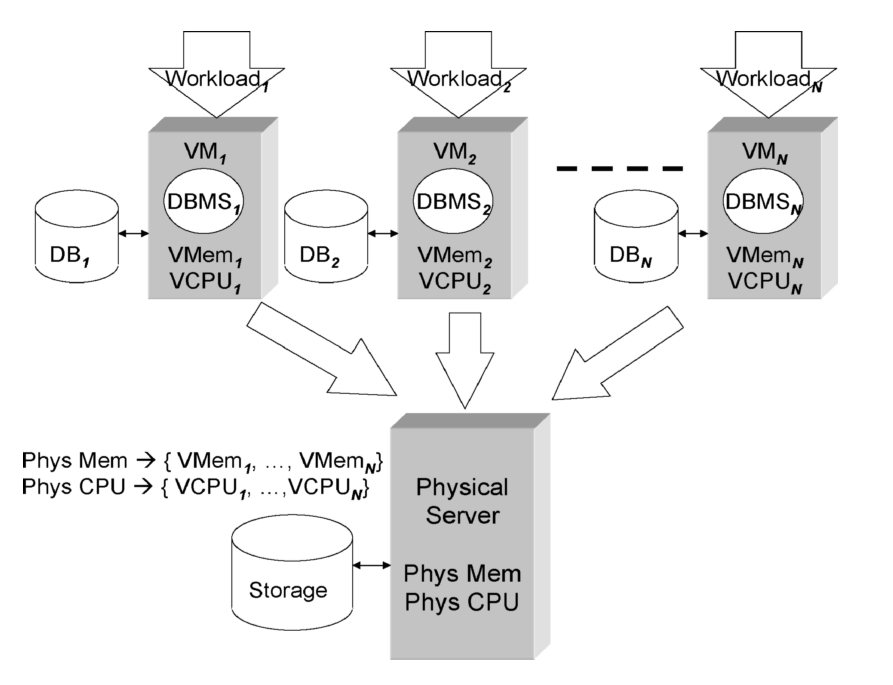
\includegraphics[width=0.8\textwidth]{dbms_consolidation.png}
\caption{Resource Consolidation scenario}
\label{fig:scenario}
\end{figure} 

\section{Problem definition}

In order to model this problem, the author assumes that there are  $M$ types of resources , such as CPU capacity, memory, or I/O bandwidth. The notation used to represent the share of resources allocated to a VM running a workload $W_{i}$ is $R_{i} = [r_{i1},...r_{iM}], 0 \leq r_{ij} \leq 1$. This workload represents the statements processed by the different DMBS instances at the same amount of time. 

Each workload has a cost, which depends on the resource share allocated to the VM in which it runs. It is used $Cost(W_{i},R_{i})$ to represent the cost of running the workload $W_{i}$ under resource allocation $R_{i}$. Considering that there are $N$ workloads, the goal is to choose $r_{ij}, 1 \leq i \leq N, 1 \leq j \leq M$ such that 
\[
  \sum_{i=1}^{N} Cost(W_{i},R_{i})
\]
is minimized.

This problem is generalized to satisfy Quality of Service (QoS) requirements.On of these requirements is to specify the maximum increase in cost that is allowed for a workload under the recommended resource allocation. It was defined a \textit{cost degradation} as
\[
 Degradation(W_{i},R_{i}) = \frac{Cost(W_{i},R_{i})}{Cost(W_{i},[1,...,1])}
\]
, where $[1,...,1]$ represents the resource allocation in which all the available resources are allocated to $W_{i}$. It can be specified a \textit{degradation limit} $L_{i} ( L_{i} \geq 1 )$, such that 
\[
 Degradation(W_{i}, R_{i}) \leq L_{i}
\]
for all $i$. This limit is set per workload, so it does not need information about other workloads that it will be sharing the physical server with.

The other QoS requirement introduced is the ability to specify relative priorities among the different workloads. A \textit{benefit gain factor} $G_{i} (G_{i} \geq 1)$ can be used to indicate how important is to improve the performance of $W_{i}$. Each unit of improvement is considered to worth $G_{i}$ cost units. When this parameter is applied to the problem, it may cause a workload to get more resources than its fair share. In order to incorporate it to our problem, the cost equation is modified to minimize the following
\[
  \sum_{i=1}^{N} G_{i} * Cost(W_{i},R_{i})
\]


\section{Architecture}

The process of  determining the allocation of resources to each VM is not immediate, nor static. The proposed advisor follows a sequence of steps. Initially, it makes resource allocations based on the workload descriptions and performance goals, which is performed offline, i.e., the VMs are not running yet. Then two following steps are performed online. First, it adjusts its recommendations based on workload costs to correct for any cost estimation erros made during the initial phase. Second, it uses continuing monitoring information to dynamically detect changes in the workloads. This last step is important because a workload cannot be considered static, its resource needs may change during execution. This approach prevents the advisor from allocating resources to DBMS instances that will obtain little benefit from them.

Since the advisor has a considerable number of sub-processes, it makes sense to organize it in modules. An overview of this advisor in a modular way is given in ~\ref{fig:architecture}. This paper intends to give a brief explanation of each module.


\begin{figure}[ht]
\centering
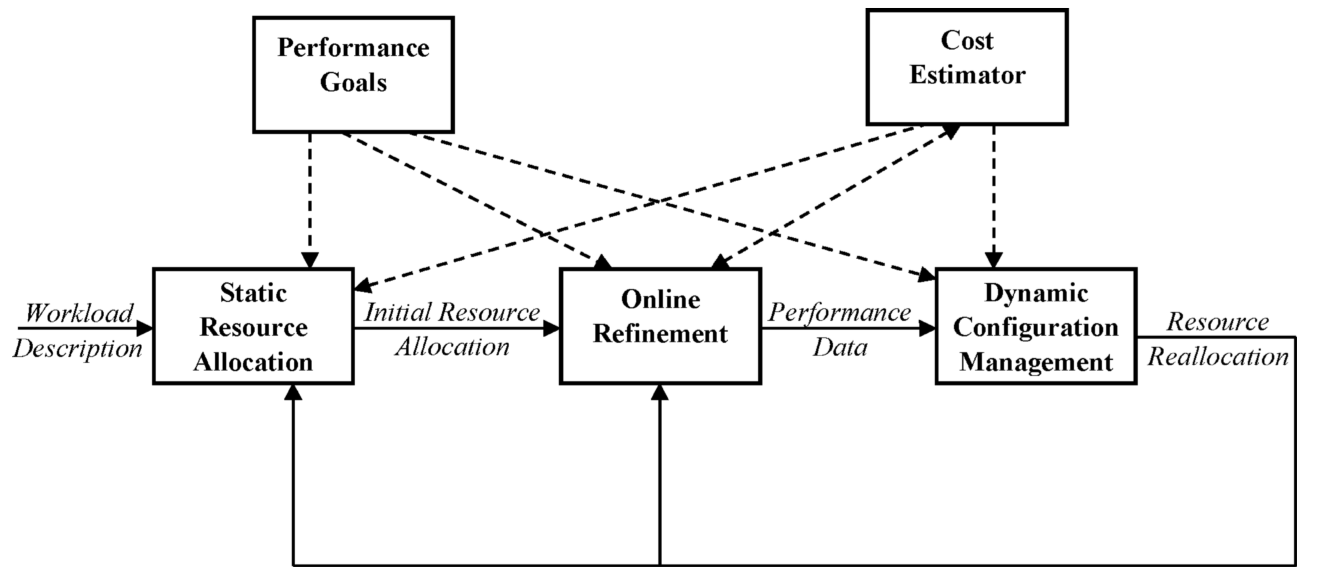
\includegraphics[width=0.8\textwidth]{architecture.png}
\caption{Advisor overview}
\label{fig:architecture}
\end{figure} 

\subsection{Cost estimation and initial allocation}

Given a workload $W_{i}$, the cost estimator will estimate $Cost(W_{i},R_{i})$. The strategy used to implement this module is to leverage the cost models built into database systems for query optimization. The query optimizer cost model can be described as $Cost_{DB}(W_{i},P_{i},D_{i})$, where $W_{i}$ is a SQL workload, $P_{i} = [p_{i1},..,p_{iL}]$ is a vector of parameters that are used to list both the available computing resources and DBMS configuration parameters relevant to the cost model, and $D_{i}$ is  the database instance. 

The author identifies two problems in using only query optimizer cost models. The first problem is the difficulty of comparing cost estimates produced by different DMBSes. They may have different cost models. Even if they share the same notion of cost, they normalize costs differently. This problem is addressed partially by the advisor. Although it only considers that the DBMSes have the same notion of cost, it proposes a renormalization step, in order to make $Cost_{DB}(W_{i},P_{i},D_{i})$ from different DBMSes comparable. For our purpose this step is not considered for implementation, since the support of multiple DBMSes is out of scope of this paper.

The second problem is that the query optimizer cost estimates depends on $P_{i}$, while the virtualization design advisor is given a candidate resource allocation $R_{i}$. The mapping of these two parameters is done through a calibration step. This step determines a set of DBMS cost model configuration parameters according to the different possible candidate resource allocations. It is supposed to be performed per DMBS on the physical machine before running the virtualization design advisor. Once the appropriate configuration parameters $P_{i}$ are determined for every possible $R_{i}$, the DBMS cost model is used to generate $Cost_{DB}$.

The calibration step is performed on  \textit{descritive parameters}, which are used to characterize the execution environment. The approach to the \textit{prescritive parameters}, which control the configuration of the DBMS itself, is to leave it for user definition. For instance, the ~\ref{table:descritive}  show some descritive parameters used in PostgreSQL, while ~\ref{table:prescritive}  show the prescritive ones. 


\begin{table}[ht]
    \centering
    \begin{tabular}{ | l | p{5cm} |}
    \hline
    Parameter & Description  \\ \hline
    \textbf{random\_page\_cost} & Cost of non-sequential page I/O \\ \hline
    \textbf{cpu\_tuple\_cost} & CPU cost of processing one tuple \\ \hline
    \textbf{effective\_page\_size} & size of file system's page size  \\
    \hline
    \end{tabular}
    \caption{Descritive parameters}
    \label{table:descritive}
\end{table}


\begin{table}[ht]
    \centering
    \begin{tabular}{ | l | p{5cm} |}
    \hline
      Parameter & Description  \\ \hline
    \textbf{shared\_buffers} & shared bufferpool size \\ \hline
    \textbf{work\_mem} & amount of memory used by each sort and hashing operator. \\
    \hline
    \end{tabular}
    \caption{Prescritive parameters}
    \label{table:prescritive}
\end{table}

The calibration follows the basic methodology for each parameter $p_{ij} \in P_{i}$:

\begin{itemize}
 \item (1) Define a calibration query $Q$ and a calibration database $D$, such that $Cost_{DB}(Q,P_{i},D)$ is independent for all descritive parameters in $P_{i}$, except for $p_{ij}$; \\
  \item (2) Choose a resource allocation $R_{i}$, instantiate $D$, and run $Q$ under that resource allocation, and measure the execution time $T_{Q}$; \\
  \item (3) This step refers to the renormalization of the $Cost_{DB}$ provided by the DBMS. As mentioned earlier in this section, we are not going into the details of this step; \\
  \item (4) Repeat the two preceding steps for a variety of $R_{i}$, associating with each  a value of $p_{ij}$, which describes a certain resource. For instance, query optimizer parameters that describe CPU, I/O and memory are independent of each other and can be calibrated independently; \\
  \item (5) Perform regression analysis on the set of $(R_{i},p_{ik})$ value pairs to determine a calibration function $Cal_{ij}$ that maps resource allocations to $p_{ik}$ values. \\
\end{itemize}

During the described methodology, calibration queries should be carefully chosen. They need to be dependent only on the parameter that is being calibrated. If it is not possible to isolate one parameter, a system of $k$ equations is solved to determine the values for the $k$ parameters.


\subsection{Online refinement}

The initial allocation is based on the calibrated query optimizer cost model, as described earlier. This enables the advisor to make recommendations based on an informed cost model. However, this model may have inaccuracies that lead to sub-optimal recommendations. The  \textit{online refinement} is based on the observation the actual times of different workloads in the different virtual machines. It uses these observations to refine resource allocation recommendations. Then the advisor is rerun with the new cost models, so  we can obtain an improved resource allocation for different workloads. These optimizations are performed until the allocations stabilize. It's important to notice that the goal of the \textit{online refinement} is not deal with dynamic changes in the workload, which are dealt by another module, but to correct cost models. Thus, it's assumed that the workload is not going to change during this process. 

In order to optimize the recommendations, it is necessary to identify the cost model behaviour. The author identifies two types of models. The first is the \textit{linear model}, which can describe the allocation of CPU. For this resource workload completion times is linear in the inverse of the resource allocation level. Thus, the cost model in this case can be represented by
\[
 Cost(W_{i}, [r_{i}]) = \frac{\alpha_{i}}{r_{i}} +\beta_{i}.
\]

The values $\alpha_{i}$ and $\beta_{i}$ are obtained through a linear regression. This regression is performed on multiple points represented by estimated costs for different $r_{i}$ values used during the initial allocation phase. This cost is adjusted by two parameters, $Est_{i}$ and $Act_{i}$, they represent the estimated cost of workload and the runtime cost, respectively. When the cost is underestimated, these parameters are used to increase the slope of our cost equation. From another standpoint, when this value is overestimated, we need to decrease the slope. This is achieved by
\[
  Cost(W_{i}, [r_{i}]) = \frac{Act_{i}}{Est_{i}} * \frac{\alpha_{i}}{r_{i}} + \frac{Act_{i}}{Est_{i}} * \beta_{i}.
\]

However, not all resources are linear. The second type of cost model identified is the \textit{piecewise-linear}, which describes the allocation of memory. Increasing this resource does not consistently result in performance gain. The magnitude and the rate of improvement change according to the query execution plan. The cost equation is similar to the linear cost model, it is given by
\[
  Cost(W_{i}, [r_{i}]) = \frac{Act_{i}}{Est_{i}} * \frac{\alpha_{ij}}{r_{i}} + \frac{Act_{i}}{Est_{i}} * \beta_{ij}, r_{i} \in A_{ij}.
\]
The difference here is the parameter $A_{ij}$, which represents the interval of resource allocation levels corresponding to a particular query execution plan, that is represented by $j$. Its intervals are obtained during the initial phase, when the query optimizer is called with different resource allocations and returns different query execution plans with their respective costs. These query execution plans define the boundaries of the $A_{ij}$ intervals. The end of this interval is the largest resource allocation level for which the query optimizer produced this plan. The initial values of $\alpha_{ij}$ and $\beta_{ij}$ are obtained through linear regression. Together with $A_{ij}$, they are subsequently adjusted.

Both of the equations presented work within their cost model. Nevertheless, a physical  machine has more than one type of resource. Therefore, the author extends the cost equations to multiple resources. He deals with the case in which $M$ resources are recommended, such that $M-1$ resources can be modelled using a linear function, while the resource $M$ is modelled using a piecewise-linear function. The cost of workload $W_{i}$, given a resource allocation $R_{i} = [r_{i1},...,r_{iM}]$ can be given by
\[
  Cost(W_{i}, R_{i}) = \sum_{j=1}^{M} \frac{Act_{i}}{Est_{i}} * \frac{\alpha_{ijk}}{r_{ij}} + \frac{Act_{i}}{Est_{i}} * \beta_{ik}, r_{iM} \in A_{iMk},
\]
in which $k$ represents a certain query execution plan, which defines the boundaries of $A_{iMk}$. 

During refinement, this equation is supposed to be performed iteratively, in order to optimize the parameters $\alpha_{ijk}$ and $\beta_{ijk}$. This iteration is shown below.
\begin{eqnarray*}
 Cost(W_{i}, R_{i}) &=& \sum_{j=1}^{M} \frac{Act_{i}}{Est_{i}} * \frac{\alpha_{ijk}}{r_{ij}} + \frac{Act_{i}}{Est_{i}} * \beta_{ik} = \sum_{j=1}^{M} \frac{\alpha'_{ijk}}{r_{ij}} + \beta'_{ik}, r_{iM} \in A_{iMk} \\
 Cost(W_{i}, R_{i}) &=& \sum_{j=1}^{M} \frac{Act_{i}}{Est_{i}} * \frac{\alpha'_{ijk}}{r_{ij}} + \frac{Act_{i}}{Est_{i}} * \beta'_{ik} = \sum_{j=1}^{M} \frac{\alpha''_{ijk}}{r_{ij}} + \beta''_{ik}, r_{iM} \in A_{iMk} \\
  &\vdots&
\end{eqnarray*}

The author in \cite{Soror:2008:AVM:1376616.1376711} proposes an heuristic that changes the equation in the first iteration. Instead of  considering the interval $A_{iMk}$, the first iteration scales all the intervals of the cost equation (i.e., for all $k$). This is done because the estimation errors may reside in a bias in the query optimizer's view of resource allocation levels. In the second iteration and beyond, this cost will be refined according to the interval $A_{iMk}$, where the resource $r_{iM}$ will be scaled.

These refinement iterations will stop under two situations. The first is when the newly resource allocation recommendation is the same as the second. The second situation is when the refinement continues beyond $M$ iterations. In this case the refinement process continues, but through a linear regression model to the observed points. The query estimates wouldn't be necessary anymore. This process only finishes when the number of iterations reach an upper bound, placed manually. It is used to guarantee termination.

\section{Dynamic configuration management}

Even if we have an optimal resource allocation, the workload may change its behaviour during execution. They may occur due to the intensity of the workload (e.g. increased number of clients), or the nature of the workload (e.g. new set of queries with different resource needs ). These changes are not dealt by our online refinement, that's why the dynamic configuration management is needed. 

The proposed approach consists in monitoring the relative changes in the average cost per queries between periods. If the change in the estimated cost per query is above a threshold, $\theta$, we classify this a major change. When this is identified, it's decided to make the virtualization design advisor to restart its cost modeling from initial state, before online refinement. The cost model needs to be discarded, since it no longer reflects information about the workload.

In order to deal with minor changes, it's introduced a new metric $E_{ip}$. It represents the relative error between the estimated and the observed cost of running workload $W_{i}$ in monitoring period $p$. We analyze two consecutive periods. If both $E_{i(p-1)}$ and $E_{ip}$ are below some threshold ( e.g. $5\%$ ), or if $E_{ip} - E_{i(p-1)} > 0$, then we continue with online refinement. In this case, the erros are either small, or are decreasing. Both of these situations can be effitiently dealt by some iterations of online refinement. However, if this condition is not satisfied, we discard the cost model again. 
\chapter{\textbf{Cloud infrastructure management}}


This section will be used to described OpenNebula, that is a virtual infrastructure (VI) manager. Organizations can use it to manage and deploy VMs, individually or in groups that must be co-scheduled on local or external resources, which means that it supports hybrid clouds. Some of its key features are:
\begin{itemize}
 \item It provides a homogeneous view of resources, regardless of the underlying hypervisor (e.g. KVM, Xen). This makes the virtualization much less restrictive. The physical machine in which the VM is being run does not need to be tied to a specific virtualization technology, causing incompatibility issues;
  \item Manage a VM's full life cycle, like managing storage requirements and setting up the network;
  \item Supports configurable resource allocation policy.
\end{itemize}

The OpenNebula architecture is illustrated by ~\ref{fig:open_arch}. It basically can be split into three layers. The core (middle layer ) has three management areas. One of them is dealing with the creation of virtual networks, which is done through the Virtual Network (VN) manager. This component keeps track of leases ( a set form by one IP and one MAC address valid on a particular network ), and their associations with VMs and physical bridges they are using. Second, it needs to manage and monitor the physical, which is responsibility of the host manager. And finally, there is the VM manager, responsible for taking care of a VM's life cycle. It prepare the disk images for them, by controlling the image and storage technologies. It also needs to control the hypervisors, for creating and controlling them. And combined with the VN manager, it provides the VM with the network environment. These managers count with a SQL Pool, which saves the OpenNebula state, and in case of a failure, it is possible to restore it.

\begin{figure}[ht]
  \centering
 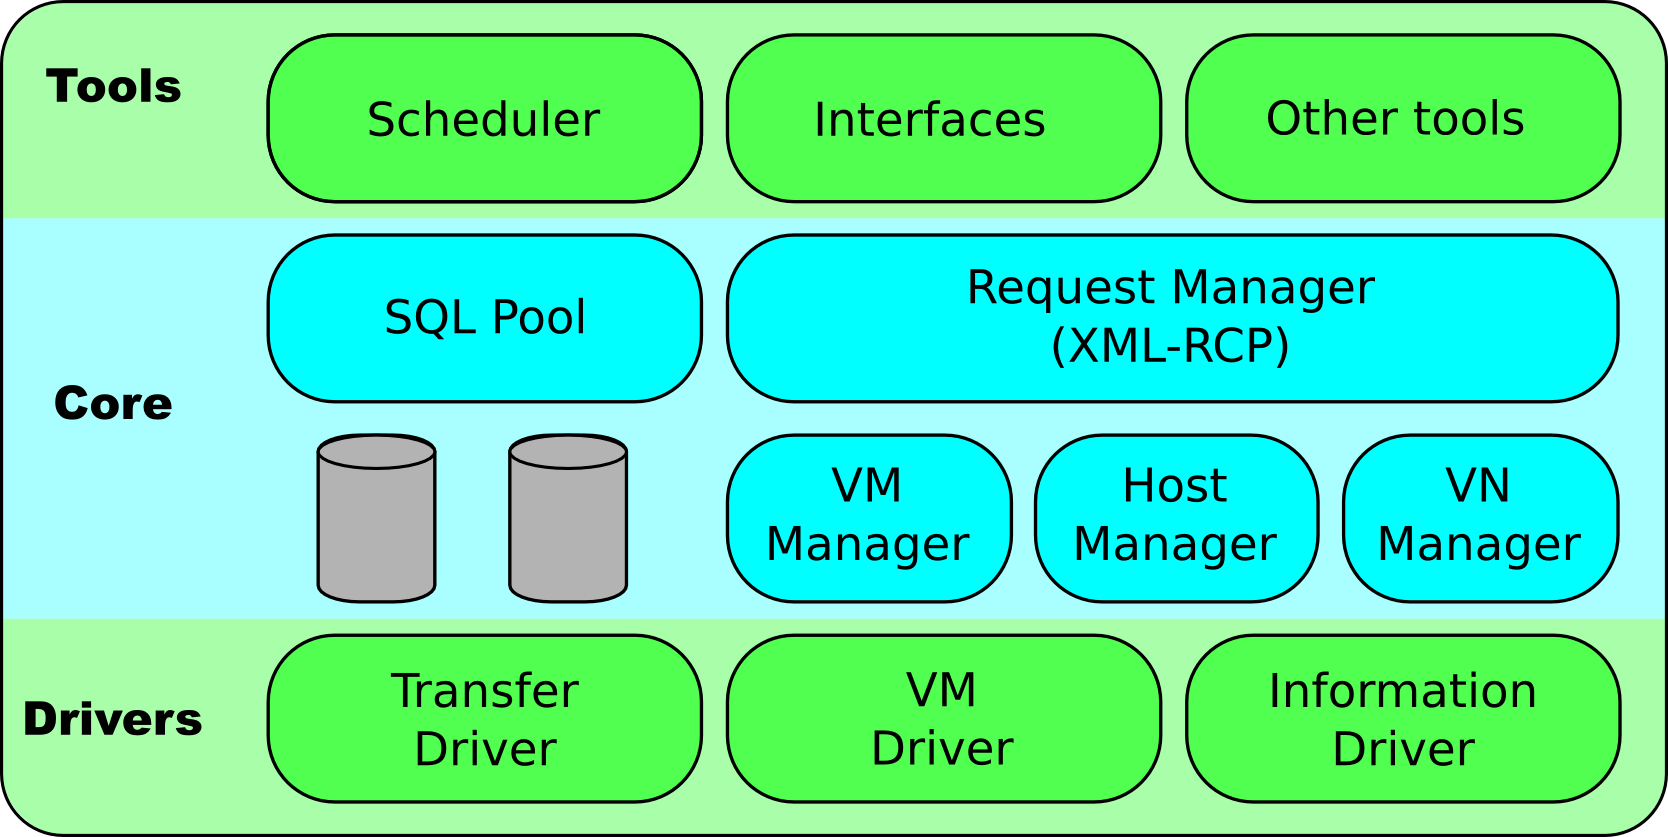
\includegraphics[scale=1]{one-architecture.png}
  \caption{OpenNebula architecture}
  \label{fig:open_arch}
\end{figure}

One important feature of the core module is the support of service deployment. The Request manager exposes a XML-RPC interface that decouples most of the functionality present in the core. As OpenNebula is in continuing development, it is expected that this API will support even more functionality. Currently, it is known that dynamic resource allocation is not supported yet. We'll discuss this issue on the next section, as this functionality is important for the advisor.

All these described activities are performed through pluggable drivers, present in the bottom layer. This modularity makes the system easier to extend and avoids tying it to any specific technology. The drivers shown in ~\ref{fig:open_arch}  address some particular areas, such as virtualization ( by controlling the hypervisor ), storage operations, gather monitoring information and authenticate user requests.

In the top layer tool there are both user interfaces to access OpenNebula, but also APIs extended from the XML-RPC, which can work between the core and other tools. Even more relevant for this paper is the OpenNebula's scheduler, also in this layer. Its job is to make VMs placement decisions, i.e. it assigns physical machines for VMs. It has access to all requests OpenNebula receives. Based on these requests, it keeps track on allocations and sends the appropriate deployment commands to OpenNebula core. As other modules, it can be replaced by third party solutions, such as Haizea\footnote{http://haizea.cs.uchicago.edu/},  which offers more sophisticated placement policies. However, in this paper we will stick to the OpenNebula's default scheduler.

The scheduler already present in OpenNebula works only with immediate provisioning. Its concept is pretty straightforward, the resources are only provisioned at the moment they are required, if that's not possible, then the requirement is ignored. The requirements are done in a manual and static way, in which amount of resources, among other configurations, are defined in a file. The assignment is performed through a classification policy.  The administrator needs to set a \textit{RANK} variable, which defines which host is more suitable to host a VM. Each VM has its own \text{RANK}, and the scheduler assigns will assign a host with the highest value for this variable to a VM. It's possible to define a VM template in OpenNebula, so you can share the same scheduling policy  to a group of VMs. For instance, here are some possible \textit{RANK} definitions, each one serving a specific policy:

\begin{itemize}
 \item Load-aware Policy
 \begin{itemize}
   \item \textbf{Heuristic:} Use nodes with less load;
   \item \textbf{Implementation:} Use nodes with more \textit{FREECPU} first.
    \item \textit{RANK} = \textit{FREECPU}

 \end{itemize}

  \item Striping policy
  \begin{itemize}
   \item \textbf{Heuristic:} Spread the VMs in the cluster node;
   \item \textbf{Implementation:} Use the nodes with less VMs running first.
   \item \textit{RANK} = "\textit{- RUNNING\_VMS}"
  \end{itemize}

\end{itemize}


\chapter{\textbf{Implementation}}



\chapter{\textbf{Proposed implementation}}

In this paper, it's proposed an implementation of the virtualization design advisor over OpenNebula. The aim is to optimize the distribution of resources inside the private part of a cloud for VMs running database workloads. Since it's not possible, nor makes sense to optimize an external provider's infrastructure, the public part of the cloud is just ignored. We also stick to the PostgreSQL\footnote{http://www.postgresql.org/} as the DBMS used in our solution, although the support for other DBMSs could be extended in future work.

As already described, the virtualization designer advisor has only been modelled and tested against one server. There are two issues in porting this solution to a cloud. First, a cloud can contain several hosts, instead of one. Other issue is that a cloud is a heterogeneous environment. In spite of the homogeneous view of resources provided by the VMM, the hosts may be different themselves. To address these problems, the proposed approach consists in having $N$ instances of our advisor, being $N$ the number of nodes in the private cloud. Therefore, the advisor will not see the cloud as a whole, but only the host it was assigned to work with, the same as it was working with only one server. 

The first step of this implementation would be the creation of a module responsible for the calibration process. As discussed earlier, this calibration will be used to map the query optimizer's cost model, which depends on its parameters $P_{i}$, to  the advisor's cost model, based on resources $R_{i}$. This process is supposed to be executed before any VM deployment, since the initial allocation depends on the latter cost model. Thus, it will be executed whenever a new physical host is added to a cluster. As this paper is limited to one DBMS, the renormalization step will  not be performed.


After calibration, we expect the OpenNebula's default scheduler to define which host will be assigned to the VM that is to be deployed, as usual. At this step, the only provision that needs to be taken is to set the \textit{RANK} variable properly. In this paper, we intend to deal with only two types of resources: memory and CPU. Therefore, we propose the following heuristic for the \textit{RANK}:
\begin{itemize}
 \item \textit{RANK} $=$ $\alpha *$ \textit{FREECPU} + $ (1 -\alpha) *$ \textit{FREEMEMORY}, $  0 \le \alpha \le 1  $.
\end{itemize}
In this equation, we expect $\alpha$ to be used to prioritize one type of resource over another. Since the scheduler assigns the host before being possible to run the advisor, this heuristic will be used for all kinds of workloads. So it doesn't matter whether they are more or less CPU intensive or memory intensive. We consider this to be a limitation. However, we still expect that this heuristic will be able to  distribute well the VMs among the hosts.

Once the VMs are placed on a machine, the initial configuration step from the virtualization design advisor can be started. In order to deal with their initial configuration, it's proposed the use of the greedy search algorithm, described earlier in this paper. A problem that has already been identified, which affects the greedy algorithm, is the lack of current support for dynamic resource reallocation in OpenNebula. One possible approach would be the use of libvirt\footnote{http://libvirt.org/}, which defines itself as "A toolkit to interact with the virtualization capabilities of recent versions of Linux (and other OSes)". It offers an API that works with all the hypervisors supported by OpenNebula, offering many features, including resource reallocation. Currently, OpenNebula has an libvirt API, which enables this tool to manage the VMs over the core layer. It should be possible to implement a solution by using libvirt under the core layer, to extend the drivers' capabilities too.

The online refinement and the dynamic configuration management steps should have direct implementations, following their descriptions. The initial configuration is defined by the greedy algorithm ( the static resource allocation module ), it stops when it finds the best allocation, which may be the optimal or close to it. Once this task is performed, the online refinement is started. It updates the cost model by observing estimated and actual times of workloads.  It returns an optimized cost model to the first step, where the greedy algorithm is restarted and searches for a new recommendation with the optimized cost model. The optimizer only stops when the newly obtained recommendations don't differ from the original ones (i.e. it stabilizes ). The dynamic configuration management module is also started after the the end of the initial configuration. It also uses optimized cost models to monitor changes in the workload. It may restart the workload when major changes are detected.

The performance of this advisor is expected to improve as optimized cost models are obtained, and so less calls to the DBMS's query optimizer are needed. This is due to the fact that these calls have a high computational cost.



\chapter{\textbf{Final considerations}}

In this paper, it was considered the problem of automatically configuring multiple virtual machines, which were deployed in a cloud. The aim was to show that it is possible to improve the overall performance of running database workloads by optimizing the resource allocation among them. Through the development of an advisor and further experimentations, it was demonstrated that this objective can be achieved even by reallocating a single resource.

Our approach to leverage the cost model built within the query optimizer was shown to be effective. The advantage of its use is that the cost model takes into consideration the nature of database workloads. However, this approach can turn the support of new DBMSes much harder. If a DBMS does not offer tools for self calibration, the tuning parameters that describe its resources must be calibrated manually. Thus, their use within the cost model and their variation need to be analyzed. For the same reason, the support of new resources are also hard.

We have also shown that without the advisor, all resource allocation levels must be set manually and they are static along the VM's life cycle. This means that they will not be adapted to the workload needs. That is why the existence of the virtualization design advisor in a cloud is important.

There is a lot of room for future work in database consolidation. Obvious directions include expanding the virtualization design advisor, in order to support new resource types and DBMSes. In addition, further experiments could show the effects of changing the workload intensity when running the workloads.

Furthermore, the cloud infrastructure could be more exploited. In this work, we tried to improve the performance of the database workloads by optimizing the resource reallocation inside each host from the cloud. This means that the advisor does not see the cloud as a whole, because it does not need to. In future implementations, VM migration could be used to transfer VMs to hosts with more available resources.  This feature is already supported by OpenNebula. The problem is how to optimize these transfers, because they generate a high overhead. 

%Even though OpenNebula's capabilities of scheduling enables a way of distributing resources, this is not enough for consolidating them. Its goal is not to analyse the application workload inside a VM. That's why the resources need to be required in a static way, in which it's not possible for them to be reallocated.

%The virtualization design advisor is a way of distributing these resources by considering the database workload. Although it generates overhead, it provides a way of dealing with both over- and under- utilization of resources. 


%For a future work, the cloud infrastructure should be more exploited. Through live migration of VMs, a technology already supported by most hypervisors and OpenNebula, it's possible to transfer VMs from one host to another. This could be useful in cases which avoiding over-utilization of resources is not possible ( e.g. too many VMs with high CPU needs in a host ). This paper was limited to deal with the problem of resource consolidation inside each host. By considering other hosts into our model, it could be possible to broaden the allocation alternatives. Then the problem would be expanded to deal with server consolidation.
%\input{capitulo6.tex}
%\input{anexo1.tex}     % se houver anexo



\nocite{*}
\bibliographystyle{plain}
\bibliography{tg}
% utilize macros (3 primeiras letras do mes em ingles, minusculas) no seu
% .bib para atribuir o nome do mes em portugues nas referencia,
% se o style for brazil, outros estilos tambem aceitam estas macros
% Ex:
%
% @InProceedings{teste,
%   author =       {Luciano}
%   year =         {2000}
%   month =        {}#sep;
% }
%
\addcontentsline{toc}{chapter}{\MakeUppercase{References}}

\singlespacing
\makecapadissertacao

\end{document}
